\section{研究背景}

% 2 页

\subsection{现有的网络路由数据集}

现有的互联网络路由数据集通常是由中立机构收集和发布的,借助分布式的收集系统和路由反馈会话,此类机构能够从互联网上不同的位置收集全球路由表中的实时 BGP 信息,并将其制作为格式化的数据库进行发布。

由于 BGP 路由条目是以路径的形式呈现,从单个或少数几个自治系统的路由表中获得的路由信息是极为有限的,同时由于最短路径原则在路径上的体现是一类最小/次小生成树结构的叠加,据此构建的图样本将以采样中心呈现类树状结构,不具有普通性,也不是本研究的研究目标。因此,本文只关注以下具有更加广泛的收集覆盖面的数据集。

RIPE RIS 是路由异常分析中一个最常见的路由数据来源,它由若干位于互联网交换中心的远程路由收集器(RRC) 收集和存储来自参与者通过 BGP 提供的路由数据,其中包含了来自数十个国家的上万个自治系统收集的路由信息。一些路由异常预警系统采用了由该项目反馈的实时数据\citing{ripe2021routing}。

RoutesView 项目\citing{denardis2020internet}是另一个类似的大型数据采集工程,它从 1997 年以来不断收集和归档全球互联网路由表的每日快照,并在全球各地与不同规模的网络建立了 BGP 路由收集会话。

几乎所有可用的网络路由数据都使用 MRT 格式\citing{blunk2011multi},它能够完整地记录路由表中的多种路由信息,其中自治系统路径是表现拓扑结构的主要信息,而社区属性则反映了路由的优先级。

\subsection{现有数据集在图网络算法中的不足}

由于现有的数据集大多以 MRT 数据集提供,此类数据集本身是一类随机事件流,不是现成的图数据集,在实际处理上暴露出了传统的路由数据集在面对图网络算法上存在的不足。

其中影响较大的一个因素是重复数据,由于路由收集器的原理是从不同采样点的 BGP 会话中接收全量的路由信息,因此对于每一个网络都存在大量重复且拥有公共边集的自治系统路径,而这些路径的数量并非在不同网络下遵循同一分布,因而影响了图网络模型的性能。\citing{fonseca2019bgp}

同时,数据在图中的分布状况也导致了数据集在图网络中效果不佳。如图 \ref{c3_as-distance} 所示,通过抽取 RIPE RIS 的 200 个节点与其它节点的平均路径长度数据,该图展示了互联网中自治系统间的平均距离及其分布状况,即数据集构建出的图的可能直径,这直观地展现出了数据集中很大一部分网络,事实上由于相距遥远,由一个或几个形成全连接(Full Mesh)或完全图的I类自治系统分隔(图中的红色部分数据)。对于图中平均路径距离的差异可以归结为对等路由的影响,这一点将在后续模型构建中被提及。

\begin{figure}[h]
    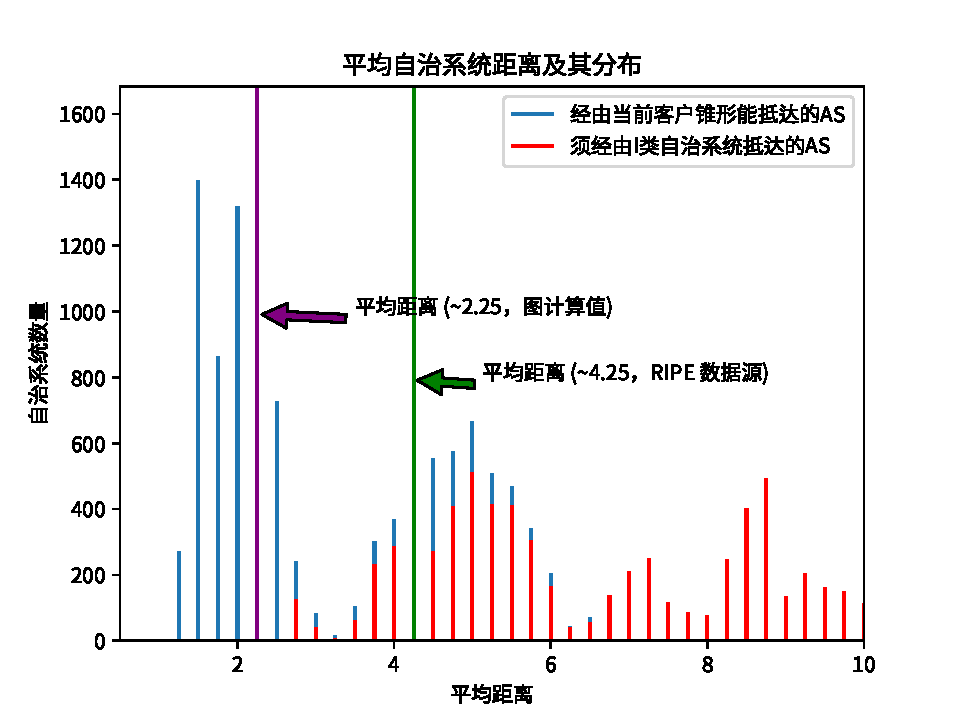
\includegraphics[width=0.85\linewidth]{chapter/c3_images/c3_as-distance.pdf}
    \caption{互联网中自治系统间的平均距离及其分布状况(RIPE RIS 数据集)}
    \label{c3_as-distance}
\end{figure}

图网络所包含的数据量也是一个值得注意的问题,事实上,据2020年一项研究报告称,全球互连网的路由数量已超过 $10^6$ 条,因而由路由数据构造的图大小本身已经超出了一些图网络模型的计算能力,这也是一些研究放弃图网络模型转而使用其它方法的原因。

此外,大部分模型研究的是特定于互联网路由表的异常检测,然而一些社区维护的分布式网络的拓扑结构与此并不相似,这类分布式网络尚未有满足本研究要求的数据集。

因而,从现有路由数据集和分布式网络出发,构建一种图网络数据集的生成算法是很有必要的。

\subsection{研究贡献}

本章从路由协议的角度出发,提出了一种新的路由数据构图方法,能够有效地去除网络中的冗余边和干扰因素,从而降低图的稠密性,使其能够在一些基于嵌入的异常检测模型下获得更好的效果,最后还使用了一些基于图网络的指标和基准算法来评估数据集的有效性,证明了它能够反映出与一般路由数据集相近的特征。